\subsection{Academic context}
The research will be based on different technologies and topics that the university has directly taught or mentioned through the degree. Specifically, we can separate this topics into four categories: radio, embedded programmable devices, network protocols and mathematical analysis.
\subsubsection{Radio}
As studied in the subjects of \href{https://fib.upc.edu/en/studies/bachelors-degrees/bachelor-degree-informatics-engineering/curriculum/syllabus/IM}{IM} and \href{https://fib.upc.edu/en/studies/bachelors-degrees/bachelor-degree-informatics-engineering/curriculum/syllabus/TXC}{TXC}, the research will focus on wireless communication, a complex topic that we are not going to study deeply but we will heavily rely upon and some knowledge is needed to effectively debug certain problems and to better understand the behavior of the system.
\subsubsection{Programmable embedded devices}
This will be the most important topic of the research as the study case will be built on microcontrollers. During the studies at the faculty, different subjects introduced the concepts of programing –\href{https://fib.upc.edu/en/studies/bachelors-degrees/bachelor-degree-informatics-engineering/curriculum/syllabus/PRO1}{PRO1} and \href{https://fib.upc.edu/en/studies/bachelors-degrees/bachelor-degree-informatics-engineering/curriculum/syllabus/PRO2}{PRO2}–, efficient data structures –\href{https://fib.upc.edu/en/studies/bachelors-degrees/bachelor-degree-informatics-engineering/curriculum/syllabus/EDA}{EDA}– and proper software design –\href{https://fib.upc.edu/en/studies/bachelors-degrees/bachelor-degree-informatics-engineering/curriculum/syllabus/IES}{IES}–. In addition, we were introduced to microcontrollers and its possible restraints –\href{https://fib.upc.edu/en/studies/bachelors-degrees/bachelor-degree-informatics-engineering/curriculum/syllabus/CI}{CI}–.
\subsubsection{Network protocols}
The research will also be heavily focused on network protocols and measuring their performance. Subjects like \href{https://fib.upc.edu/en/studies/bachelors-degrees/bachelor-degree-informatics-engineering/curriculum/syllabus/XC}{XC} provided a good introduction but \href{https://fib.upc.edu/en/studies/bachelors-degrees/bachelor-degree-informatics-engineering/curriculum/syllabus/PI}{PI} will be an essential subject as lots of the technical topics of the research were mentioned there, specifically when analyzing the LoRa mesh network.
\subsection{Terms and concepts}
%En aquest treball farem servir diverses tecnologies per a X, Y i Z. D'entre aquestes, les més significatives són A i B. Els següents apartats proporcionen una descripció i en descriuen les característiques més importants.
In this research we will use a variety of technologies and tools to fulfill the objectives described in \autoref{General objectives} in a fast and reliable way, among them, the two most significant are LoRa, a wireless communication technology, and the LilyGO T-Beam board, the hardware platform where the code and the tests will run on.
%Different technologies will help us with the research but mainly we will work with LoRa, a wireless communication technology and the LilyGO T-Beam board, the hardware platform where the code and the tests will run on.
\subsubsection{Wireless communication: LoRa}
There is different wireless communication technologies in the market, each having its strengths and weaknesses –specifically, range and throughput– and adapting to different situations and environments. \autoref{fig:TechComparative} shows, in three main categories, the different solutions available. In the short range (less than 100 m) we have RFID BLE, ZigBee, regular bluetooth and WiFi, which are designed to offer connectivity at a close range with speeds between Kbps and Mbps. In the medium range (between 100 m and 1 Km) we can also find WiFi, as some physical characteristics can allow it to reach higher ranges, and GSM technology which has a long range but is also quite power demanding. This technologies offer data rates above several Mbps. Lastly we can find SigFox, Wize, DASH7, LoRa, nWave or NB-IoT as long range (above 1 Km) communication technologies. These belong to the Low Power, Wide Area Network (LPWAN) group, which offer long range communications with a low power budget, however, this long range link comes at the expense of low data rates, in the Kbps order. However, this is often enough for IoT projects in which little data needs to be transmitted (for example, a weather measuring station) and long battery life takes precedence.
\begin{figure}[h]
        \centering
        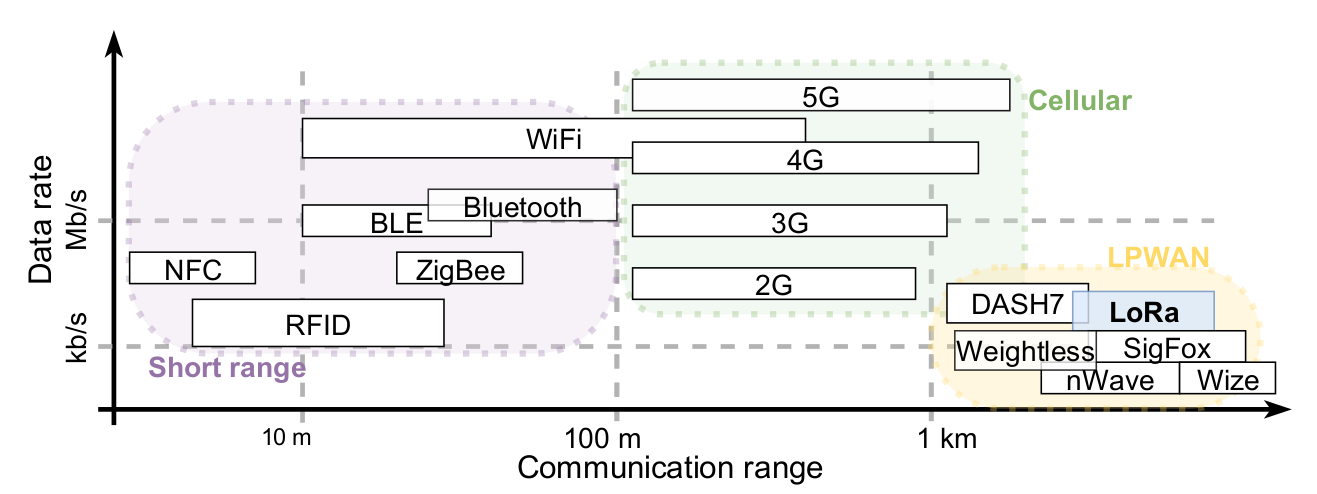
\includegraphics[height=4cm]{Figures/TechComparative.png}
        \caption{Comparison between different wireless communication technologies.}
        \cite{StarOfStars}
        \label{fig:TechComparative}
\end{figure}


LoRa, which stands for \textit{long range}, is a wireless communication technology owned by Semtech that operates in the sub-gigahertz range of the radio spectrum, specifically in the license-exempt Industrial, Scientific, Medical bands (ISM). It employs Chirp Spread Spectrum (CSS), a proprietary modulation technique resistant to multi-path fading and suitable for noisy environments, aiming to provide low throughput communication with links of more than 10 km –outdoors, in rural areas– while maintaining low power consumption.\cite{Augustin2016}

The amount of chirp that is used in the transmission is determined by the Spread Factor (SF) and this element is what makes LoRa interesting as by increasing this parameter the potential range increases at the expense of lower data throughput. 
LoRa also uses Forward Error Correction\footnote{\url{https://en.wikipedia.org/wiki/Error\_correction\_code\#Forward\_error\_correction}} (FEC) which helps with the robustness of the transmissions, specially in noisy environments.
As seen in \autoref{tab:ConfParamLoRa} LoRa is able to adapt to different scenarios by modifying its physical layer parameters: radio band and frequency, transmission power, bandwidth, FEC rate and SF although certain configurations may be against the radioelectric spectrum regulations in some jurisdictions.

\begin{table}[]
\centering
\begin{tabular}{|c|c|}
\hline
Configurable parameter & Values                    \\ \hline
Radio band             & 169, 433, 868, 915 MHz$^{a}$  \\ \hline
Bandwidth              & 62.5, 125, 250, 500 kHz$^{b}$ \\ \hline
Transmission power     & 14 dBm (EU), 27 dBm (USA) \\ \hline
Spreading Factor       & 6 to 12$^{c}$                 \\ \hline
FEC rate               & 4/5, 4/6, 4/7, 4/8        \\ \hline
\end{tabular}
\caption{Configurable parameters in LoRa transmissions \\
$^{a}$  Common frequency allocations for ISM in different regions worldwide; LoRa may also be used in licensed bands. \\
$^{b}$  Smaller bandwidths (7.8 to 41.7 kHz) are also supported, although rarely used. \\
$^{c}$  Certain bandwidth and SF combinations may result in too long transmissions for specific radio bands in which time-on-air limitations often apply.}
\label{tab:ConfParamLoRa}
\cite{StarOfStars}
\end{table}

Because LoRa is just a physical layer solution, LoRaWAN was invented to provide the MAC layer with a star topology, in which the regular nodes transmit their data in a single hop to the LoRaWAN gateway which in turn transmits it to the cloud through regular TCP/IP so the data can be later processed, be it for mathematical analysis or to distribute it to other nodes. This topology has several advantages, but also some inconvenients, as all the nodes that want to have connectivity need to be in physical range of a gateway, which will sometimes be technically or economically inviable.





%The reason that we chose LoRa for this subject is its low power consumption, its high range and the spread availability of LoRa integrated boards in the market, which, in turn, makes it affordable and easy to develop on as well as the proven reliability of the technology.
\subsubsection{Embedded devices: T-Beam}
In situations where LoRa is a suitable candidate for the communications of a solution, it is often common as well that small and a low power device is used. Thus we need to look for embedded systems that fulfill this requirements.

A common embedded board this days is the Raspberry Pi, which offers a high performance board for its size with the arm CPU architecture. It is also cheap –between 10 and 40\euro \ a piece, depending on the model– and it seems like an obvious choice to any project. However, there is some specific tasks in which a Raspberry does not perform good enough. Specifically when energy is a concern as it's estimated that it takes around 2 W\cite{PiConsumption} just to idle, and without a proper Power Management Unit (PMU) these boards also use 0.1 W when they are supposed to be shut down in addition to not support a proper sleep mode so they can we woken up later to perform periodic tasks\footnote{It is still possible to mount what's called a \textit{hat}, a physical add-on that could add the functionality of remote boot}. To put this energy measurements into perspective, a current smartphone battery would last a little bit more than half a day, thus requiring a solution to either replace the battery every one or two days –something rarely suitable– or extra hardware to provide constant energy, such as a solar cell, adding cost and complexity to the project.

Another common candidate for such tasks would be a single-board microcontroller, or what's commonly known as an \textit{Arduino}. These boards usually have lower processing power and resources but they tend to excel in the power management department which makes them great for IoT. In addition, finding one board with the exact features a project needs is relatively easy. This is the path we took. The board chosen is the TTGO T-Beam\footnote{\url{http://www.lilygo.cn/prod_view.aspx?TypeId=50033&Id=1163}}, a ESP32 SoC based board developed by LilyGo that provides us with a LoRa transceiver, WiFi+Bluetooth, a GPS as well as a hall sensor, highly programmable pins and the possibility to use a small display

\subsection{The problem}
% Aquests dos paràgrafs s'assemblen més a la "Justification" que no pas a "The problem" pero és que en certa manera tot està relacionat
During all of the history of humanity certain natural disasters have caused massive damage to properties, infrastructure, or even worse, the loss of lives; and even though predicting such events keeps being a challenging task this is not where the problems end. Rescue efforts, an extremely time critical task, and later on reconstruction work, usually rely on already existing infrastructure to assist them, but in such cases, infrastructures can not be relied upon as those probably have suffered the same fate. Thus, there is a need for a rapid deployment of critical infrastructure so relief efforts can act with the maximum efficiency without losing any second.\cite{LoRaMoto}

This is not the only use case of reliable distributed long range networks that exists. As mentioned in \cite{StarOfStars}, certain situations make it difficult to deploy a gateway close enough to a node or we would need as many gateways as nodes, which would make the use of LoRa completely pointless.


\begin{figure}[h]
        \centering
        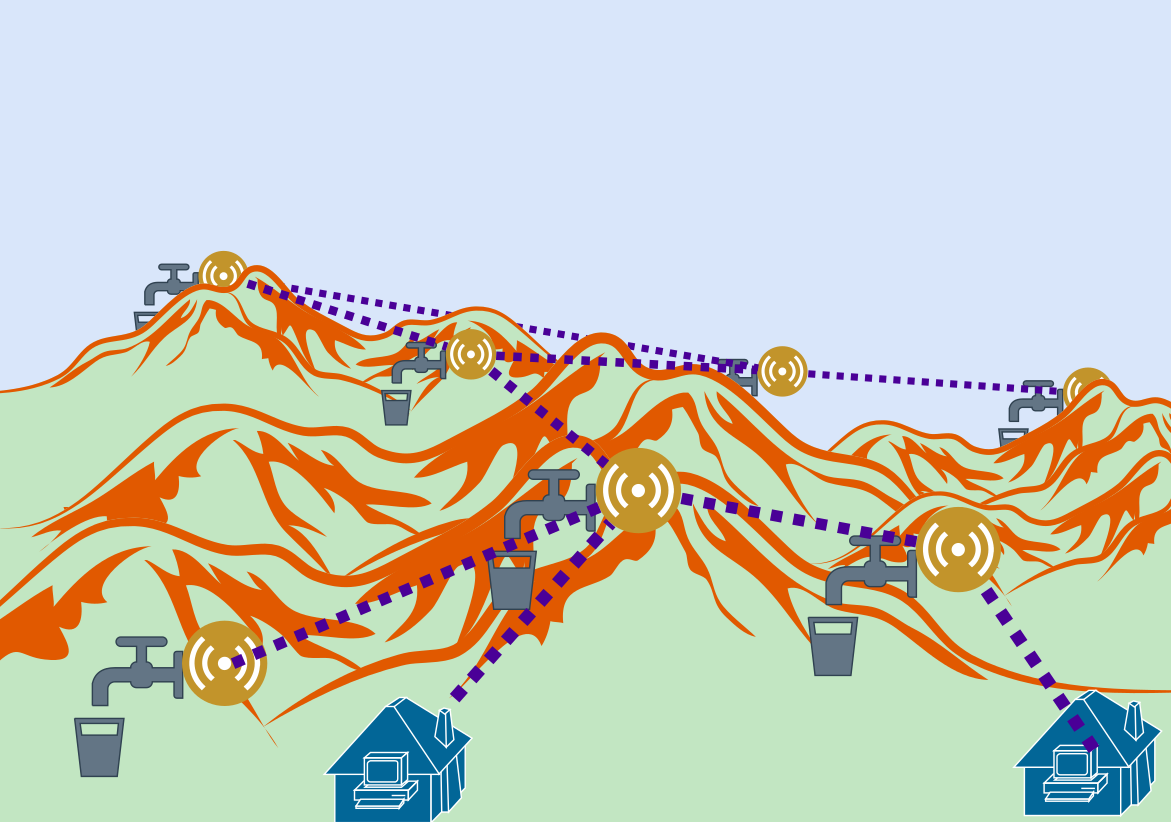
\includegraphics[height=5cm]{Figures/MountainMesh.png}
        \caption{Example of sparse network. LoRaWAN gateways would need to be installed close to every node as one gateway wouldn't be able to have a data link to many nodes.}
        \cite{StarOfStars}
        \label{fig:MountainMesh}
\end{figure}


In this cases we need to  change the paradigm, stop using the star-shaped network and use a network that is able to use all the nodes it requires to transmit data in order to be reliable and cost effective, in other words, a \textit{mesh network}, where there is no central node governing all the others and it's all the nodes that work together by forming multi-hop paths so packets get to their final destination. This technology has been already developed and a clear and practical case is Meshtastic\footnote{\url{https://meshtastic.org}}, a communication tool that leverages mesh networking and GPS data to keep people in contact in rough environments.
However, in this case we will use a networking library developed by Roger Pueyo\footnote{\url{https://dsg.ac.upc.edu/user/149/biblio}}
The research will focus on evaluating and benchmarking his network routing protocol in different environments –urban/rural, noisy/quiet, dense/sparse– and different metrics such as the network throughput, RTT, or time to settle will be measured. In addition, to measure such metrics, we will have to develop appropriate tools that are able to carry the task and we will need to fit those tools into the microcontrollers.



\subsection{Stakeholders}
The actual uses of the research are multiple and we can classify the stakeholders of the project into four categories:
\begin{itemize}
\item \textbf{End users}: This group of individuals will be the one who probably benefits of the direct results of the research and sees it applied in the field with measurable improvements on performance and reliability. It's important to acknowledge that only those projects that need networks of sensors or actuators with a big dispersion between the nodes, without the need of lots of throughput and with no direct connection to the Internet will actually benefit from that. This group includes individual civilians as well as companies and public organizations.
\item \textbf{The university, UPC}: This entity has an academic interest in this project. UPC is interested to know if it can publish the research. In addition, UPC is in charge of overseeing the documentation of this project and provides a director to ensure quality and give prover guidance. 
\item \textbf{Distributed Systems Group (UPC)}\footnote{\url{https://dsg.ac.upc.edu}}: The research will be based on Roger's work for his ongoing PhD in the DSG about developing and studying mesh networks. It will provide them information on the performance and possible areas of optimization of the protocol he designed and implemented and it will also give insight on the reliability and ensure it can be used in real world scenarios. 
\end{itemize}

%Possibles entitats que desitgin desplegar un sistema distribuit de sensors i actuadors amb baixa densitat de nodes que no requereixi un throughput molt gran i que no tinguin conexio a internet
%Els usuaris que es beneficiaran de un potencial desplegament (mes enllà de la institució)
%La UPC, perque és la universitat que porta el projecte
%En Roger, perque l'ajuda a entendre millor el protocol
